\section{Experimental evaluation}
\label{section:experiments}

We divided all experiments into two parts. In the first phase,
we have performed series of microbanchmarkings (AES encryption, 
AES decryption, RSA signature generation, RSA signature verification, 
packet processing, and database requests). Here we have measured such 
characteristics as duration and energy consumption. 
In the second phase, we have tested the overall execution of 
the system. 

\begin{figure}[!h]
	\includegraphics[width=0.5\textwidth]{graphics/demo.jpg}
	\caption{Demo setup}
	\label{fig:demo}
\end{figure}

For all primitive operations, such as encryption, decryption, hash
calculation, etc., we have measured two things: (i) duration of the
operation (in seconds); (ii) electrical current draw (in Ampers). Using duration and 
current measurements we have calculated average energy consumption as $E=UIt$.
We present the results in Table~\cite{fig:measurements}. For each experiment
we have perfomed $100$ iterations and present the mean values as results. For all operations 
we have used messages of size $1000$ bytes (for AES cipher the size of the 
message was $1024$ bytes). The operating voltage of the 
microcomputer was $5$V.

\begin{table}
	\begin{tabular}{|l|c|c|c|}
	\hline
	Operation $\downarrow$ \ Metric $\rightarrow$ & Duration (s) & Current (A) & Energy (J) \\\hline
	AES encryption (256 bits key) & $8.6\cdot10^{-5}$ & $0.16$ & $7.0\cdot10^{-5}$\\\hline
	AES decryption (256 bits key) & $7.1\cdot10^{-5}$ & $0.16$ & $5.5\cdot10^{-5}$ \\\hline
	SHA 256 hash computation & $1.3\cdot10^{-4}$ & $0.16$ & $1.1\cdot10^{-4}$ \\\hline
	RSA encryption (8192 bits modulus) & $4.2\cdot10^{-2}$ & $0.16$ & $3.4\cdot10^{-2}$ \\\hline
	RSA decryption (8192 bits modulus) & $1.1$ & $0.16$ & $9.0\cdot10^{-1}$\\\hline
	RSA signature computation (8192 bits modulus) & $1.1$ & $0.16$ & $9.0\cdot10^{-1}$ \\\hline
	RSA signature verification (8192 bits modulus) & $4.3\cdot10^{-2}$ & $0.16$ & $3.5\cdot10^{-2}$ \\\hline
	\end{tabular}
	\label{fig:measurements}
\end{table}

To measure the current we have used the setup shown in Figure~\cite{fig:current_measurement}

\begin{figure}[!h]
	\includegraphics[width=0.5\textwidth]{graphics/current_measurement_aparatus.png}
	\caption{Current measurement apparatus}
	\label{fig:current_measurement}
\end{figure}

